\section{Resumo}

A arquitetura hierárquica de veículos autônomos é comumente dividida em duas partes: alto e baixo nível. O primeiro composto principalmente por um ou mais computadores de propósito geral, que executam algoritmos que exigem alto poder computacional, e é alimentado diretamente por sensores de alto nível como câmeras, LiDARs e radares, além de receber sinais da camada de baixo nível. Esse por sua vez, é normalmente concentrado por um ou mais sistemas embarcados, que realizam a leitura de sensores de baixo nível como encoder, IMU, GPS, e fazem a atuação em motores, realizando o controle dos mesmos conforme o sinal recebido do alto nível. O Autoware é um \textit{framework} baseado em ROS que vem sendo amplamente utilizado como base do alto nível de veículos autônomos, onde por meio de um módulo de interface com o veículo, nomeado \textit{vehicle interface}, realiza a troca de dados com o baixo nível de forma transparente à natureza do mesmo. 

Porém, por meio do micro-ROS, é possível trazer o ROS para dentro do microcontrolador, dessa forma, integrando alto e baixo nível de forma implícita dentro do ecossistema ROS. Tal capacidade, permite então que a \textit{vehicle interface} do Autoware possa estar posicionada dentro do sistema embarcado, fazendo com que o \textit{framework} esteja em ambas as camadas da hierarquia de automação, e dessa forma, possa ser executado em um sistema operacional de tempo real. Dessa forma, o microAutoware é enunciado como a possibilidade de, com o apoio do micro-ROS, levar o Autoware para dentro do sistema embarcado, se comunicando com os demais nós por meio dos tópicos e serviços do ROS, sem necessidade de interromper sua arquitetura original.

Para validação da utilização da interface com o veículo dentro do sistema embarcado, foram realizadas simulações \textit{Hardware-In-the-Loop}, onde o sistema embarcado, conectado ao Autoware, foi utilizado para controlar um veículo autônomo virtual, simulado no CARLA \textit{Simulator}. Com isso, foi possível realizar os testes do \textit{hardware} sem a necessidade de um protótipo real, o que principalmente no ramo de veículos autônomos, traz além de redução de custos e tempo de testes, mais segurança para todas as pessoas envolvidas.

Dentre os recursos implementados, além de receber e enviar os dados necessários para o funcionamento do Autoware, o sistema engloba também um modo de controle manual em \textit{hardware}, utilizando um \textit{joystick}, de forma a representar por exemplo os pedais e o volante do veículo, realizando um comando indireto do carro a partir do sistema de automação. Também foram modelados protocolos de segurança para no caso de perda de \textit{deadlines} de recebimentos das mensagens do alto nível, ou do veículo (simulador), o sistema embarcado possa de forma independente passar o controle do carro para o motorista, ou entrar em modo de emergência, efetuando uma parada autônoma. Com isso, o microAutoware provou cumprir todos os requisitos de uma \textit{vehicle interface}, apresentando resultados promissores para utilização do mesmo como tal em sistemas reais.

\clearpage

\section{Motivação}

Veículos autônomos estão cada vez mais presentes nas cidades, trazendo a premissa de torná-las mais seguras, inteligentes e sustentáveis, além de trazer mais conforto aos passageiros, onde não é necessário que um deles venha a ser o motorista. A \autoref{fig:vilma} apresenta o VILMA, Veículo Autônomo do Laboratório de Mobilidade Autônoma, que por meio de uma gama de sensores e atuadores, consegue conduzir de forma 100\% autônoma.


\begin{figure}[H]
	\centering
	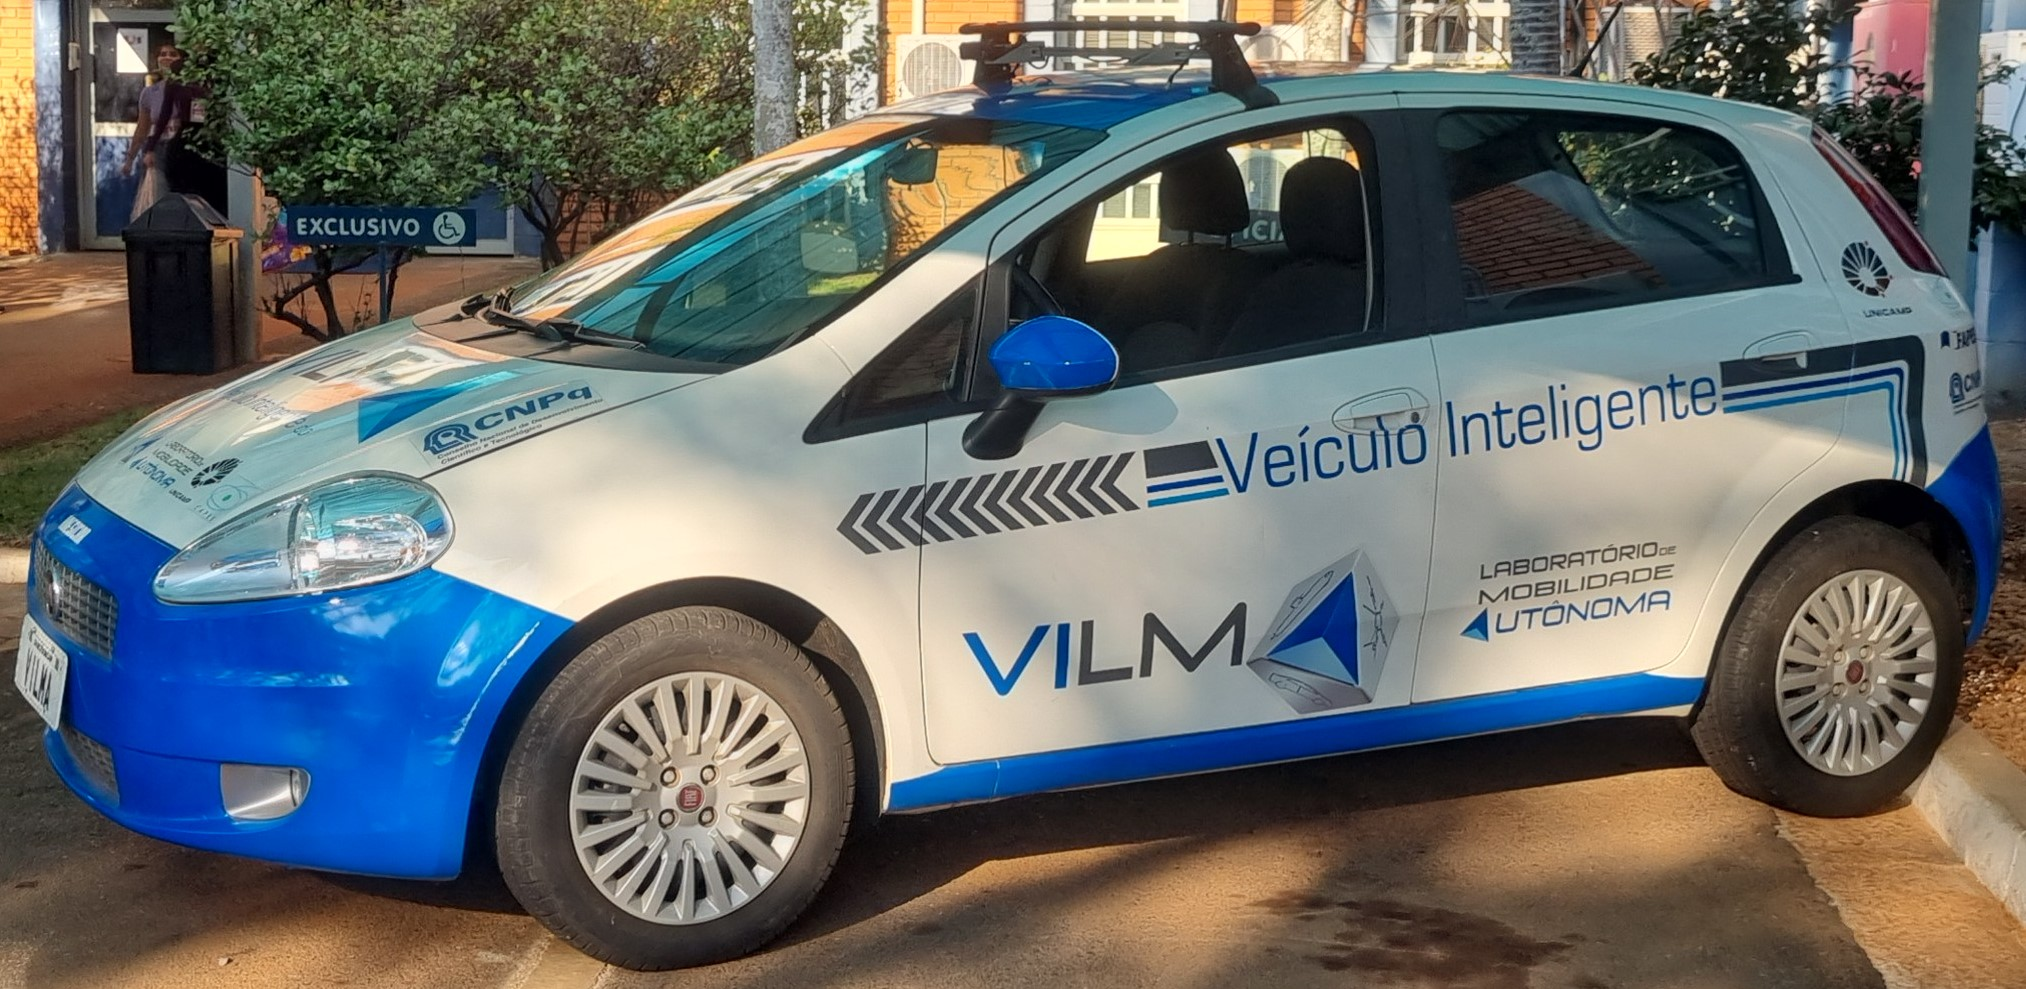
\includegraphics[width=0.5\linewidth]{img/vilma}
	\caption{Veículo Autônomo do LMA.}
	\label{fig:vilma}
\end{figure}

Parte desses sensores e atuadores são apresentados no diagrama da \autoref{fig:diagrama_vilma}, onde, os sensores de alto nível como câmera são conectados à um computador de propósito geral, e os sensores de baixo nível e atuadores são lidos e comandados por um sistema embarcado de tempo real presente no dSpace MicroAutobox. Tal sistema embarcado é uma solução comercial, de \textit{software} proprietário, ou seja, havendo necessidade da posse de licenças e personalização limitada. Por outro lado, tal sistema embarcado pode ser substituído por sistemas embarcados baseados na arquitetura ARM-Cortex, onde podem ser implementados diferentes sistemas operacionais de tempo real, dando mais liberdade e versatilidade para o desenvolvimento do baixo-nível de veículos autônomos.

\begin{figure}[H]
	\centering
	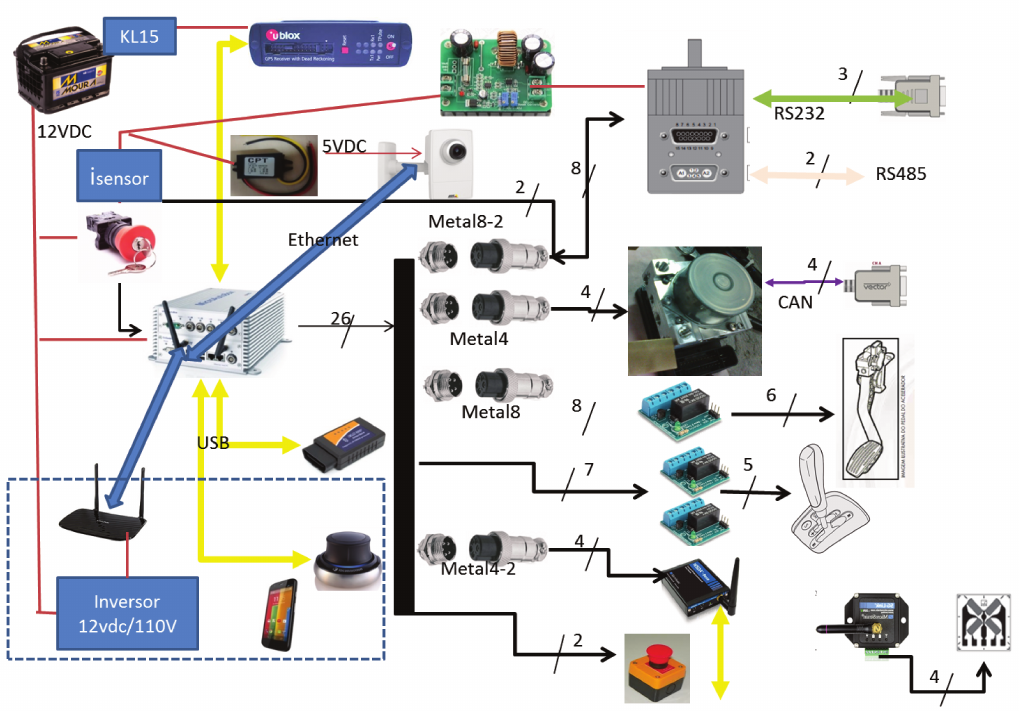
\includegraphics[width=0.75\linewidth]{img/diagrama_vilma}
	\caption{Diagrama de \textit{hardware} do VILMA01 \cite{bedoya_alise_2016}.}
	\label{fig:diagrama_vilma}
\end{figure}

Todavia, para possibilitar a condução autônoma do veículo, os itens mostrados na \autoref{fig:diagrama_vilma} e muitos outros que podem ser integrados devem ser interligados à arquitetura de automação do veículo, que normalmente é composta por módulos como percepção, planejamento, controle, localização e mapeamento. Nesse âmbito, o Autoware é um \textit{software open-source} que traz a arquitetura completa e todas as funcionalidades básicas para o guiamento de um veículo autônomo. Sua arquitetura é mostrada na \autoref{fig:hlarchitecture}, onde se percebe que a partir das entrada fornecidas pelos sensores e pelo mapa, o mesmo realiza o comando do carro a partir da \textit{vehicle interface}, que pode ser implementada de diversas formas, como por exemplo, protocolo serial ou rede CAN.

\begin{figure}
	\centering
	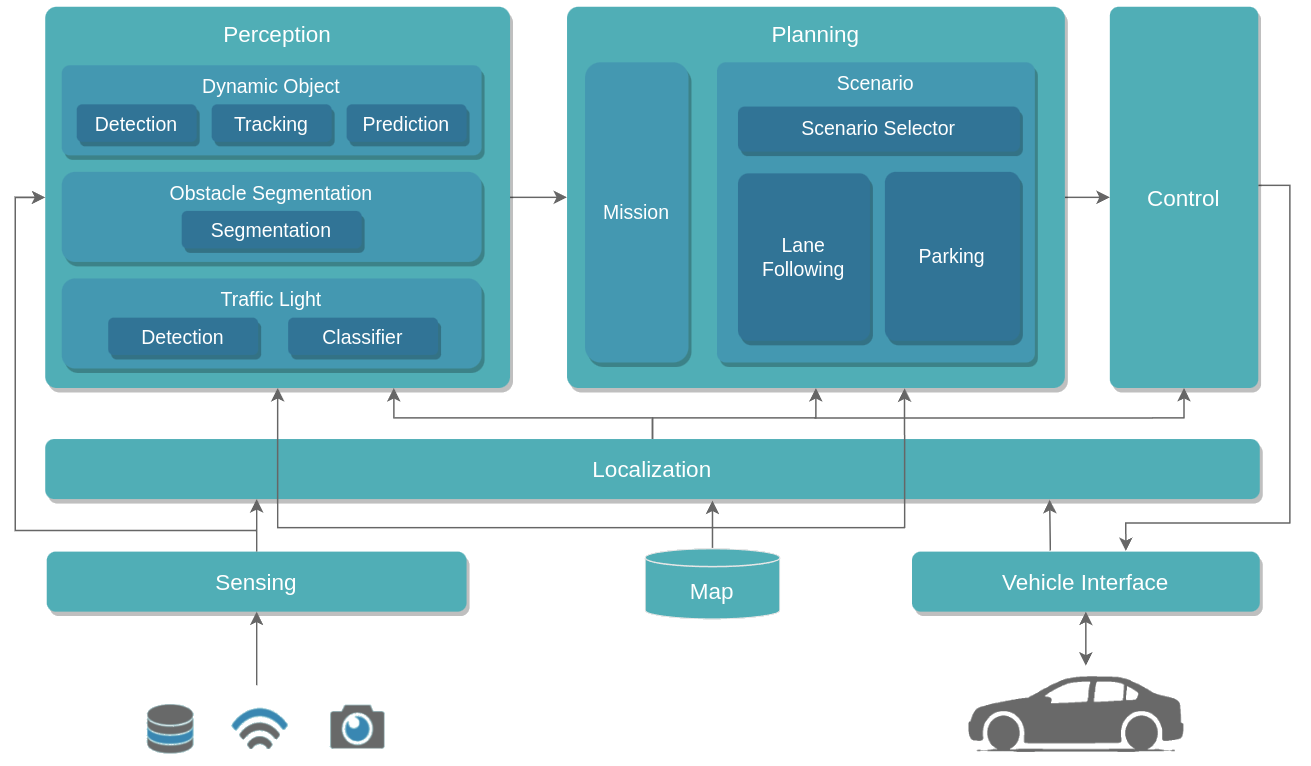
\includegraphics[width=0.8\linewidth]{img/HL_architecture}
	\caption{Arquitetura de alto nível \cite{autowareArchitecture}.}
	\label{fig:hlarchitecture}
\end{figure}

Dessa forma, o presente trabalho busca explorar a comunicação do Autoware com o veículo, por meio da utilização de sistemas embarcados de tempo real baseados na arquitetura ARM-Cortex, visando a presença do \textit{framework} em alto e baixo nível na hierarquia do veículo autônomo.


\clearpage

\section{Documentação}

A partir da problemática de integrar por meio do Autoware todos os módulos de um veículo autônomo, se mantém em aberto como será realizada a integração do sistema de alto nível do veículo com o baixo nível, que é realizado pelo módulo \textit{vehicle interface}, mas que não é especificado no \textit{framework}. Dessa forma, o escopo do projeto se define na implementação de uma interface Autoware -- veículo autônomo, como mostrado na \autoref{fig:architecture}.

Para fazer tal integração, parte-se da premissa de uma plataforma de baixo nível baseada em microcontroladores STM32, executando um sistema operacional de tempo real. A partir dessa base, propõem-se o uso do \textit{framework} micro-ROS\cite{microros_main}, para implementação do módulo \textit{vehicle interface} dentro do sistema embarcado, permitindo a presença direta do Autoware desde o alto-nível até o baixo-nível. A implementação do Autoware no microcontrolador foi batizada microAutoware.

\begin{figure}[H]
	\centering
	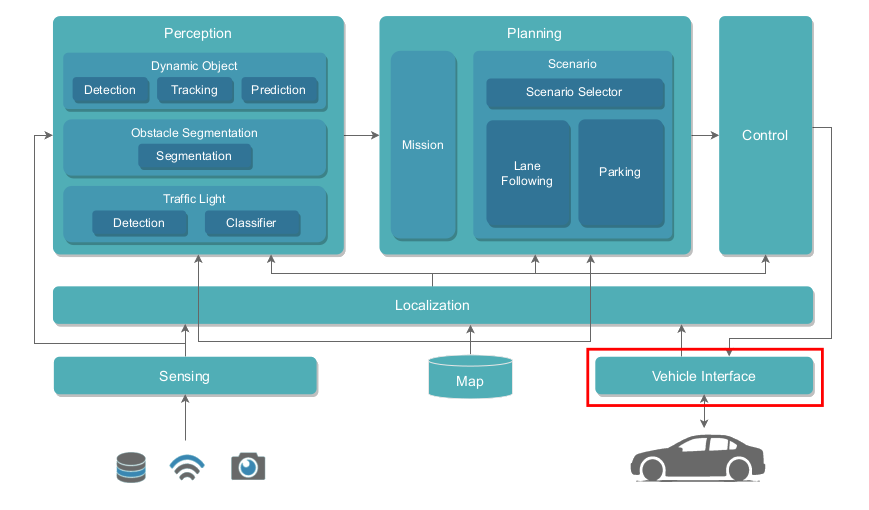
\includegraphics[width=0.75\linewidth]{img/architecture.png}
	\caption{Escopo do projeto na arquitetura Autoware.}
	\label{fig:architecture}
\end{figure}

Para realização dos testes e validação do microAutoware, foi considerada a utilização do simulador de última geração CARLA\cite{carla}, que permite que o \textit{hardware} possa ser testado sem a necessidade de um protótipo real do veículo autônomo, poupando assim: custo, risco dos equipamento e principalmente humano, e encurtando o tempo de pesquisa. Dessa forma, a validação do projeto é realizada por meio de uma arquitetura \textit{Hardware-In-the-Loop} (HIL), conforme diagrama da \autoref{fig:architecture_HIL}. Nesse cenário, o simulador representa o veículo, que alimenta o Autoware com dados de sensores de alto nível utilizados para obtenção do comando de controle que o veículo deve realizar, que é enviado para o sistema embarcado (em \textit{hardware}). Esse por sua vez, é responsável por realizar o controle do veículo no simulador, e realizar a leitura dos sensores de baixo nível do mesmo. Com isso, pode-se realizar o teste do sistema embarcado em uma estrutura que aproxima a aplicação real.

\begin{figure}[H]
	\centering
	\includegraphics[width=0.55\linewidth]{img/architecture_HIL}
	\caption{Arquitetura de teste do \textit{hardware}.}
	\label{fig:architecture_HIL}
\end{figure}

Com isso, a \autoref{fig:logos} ilustra as principais ferramentas que serão somadas ao sistema embarcado baseado em STM32 para viabilização do projeto: Autoware, ROS e micro-ROS são aliados ao CARLA para permitir a implementação e validação do microAutoware. Para integração do CARLA junto ao Autoware foi utilizada a \textit{bridge} produzida por \citeonline{kaljavesiCARLAAutowareBridgeFacilitatingAutonomous2024b}, realizando algumas modificações para integração com o microAutoware.

\begin{figure}[H]
	\centering
	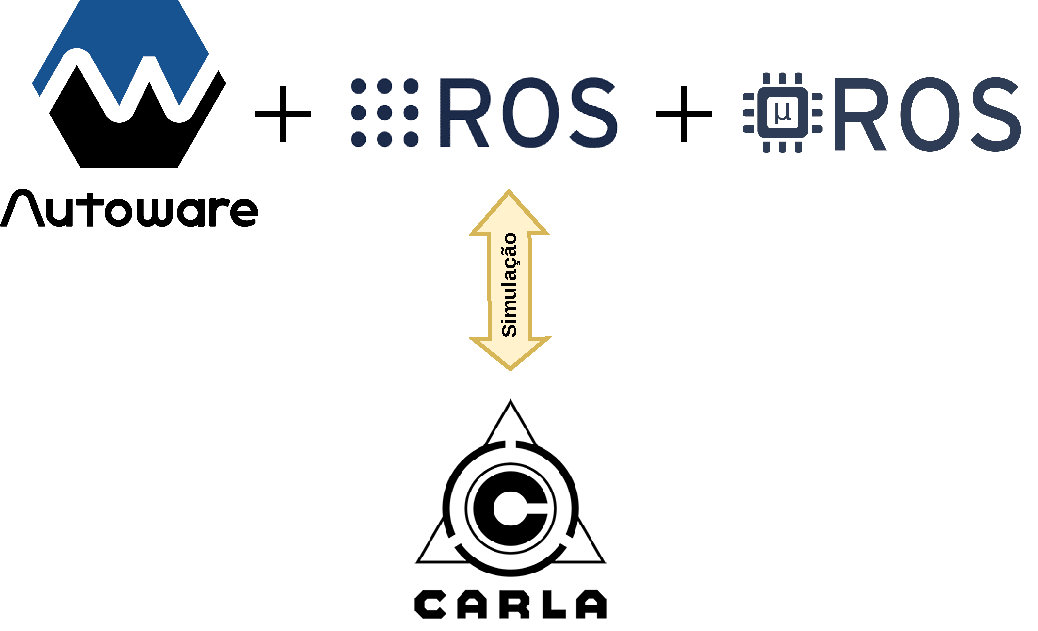
\includegraphics[width=0.75\linewidth]{img/logos}
	\caption{Ferramentas para viabilização do projeto.}
	\label{fig:logos}
\end{figure}

A \textit{vehicle interface} é um módulo que mesmo não específicado profundamente necessita de atender a alguns requisitos de comunicação, sendo eles os dados que serão recebidos (\textit{subscribers}), os dados que devem ser reportados (\textit{publishers}) e ainda um serviço de troca de modo de controle. A implementação da interface se dá por meio de um nó do ROS, que deve obrigatóriamente receber o \textbf{comando de controle} do veículo, e devolver o \textbf{modo de controle atual}, o \textbf{ângulo de esterçamento atual} e as \textbf{velocidades atuais} do veículo. Ainda, deve prover um serviço que dada uma \textbf{solicitação de troca de modo de controle}, responde se a mesma foi feita com sucesso ou não. A \autoref{fig:vehicleinterface-topics} explicita na forma de um diagrama as entradas e saídas da interface Autoware -- veículo.

	\begin{figure}[H]
	\centering
	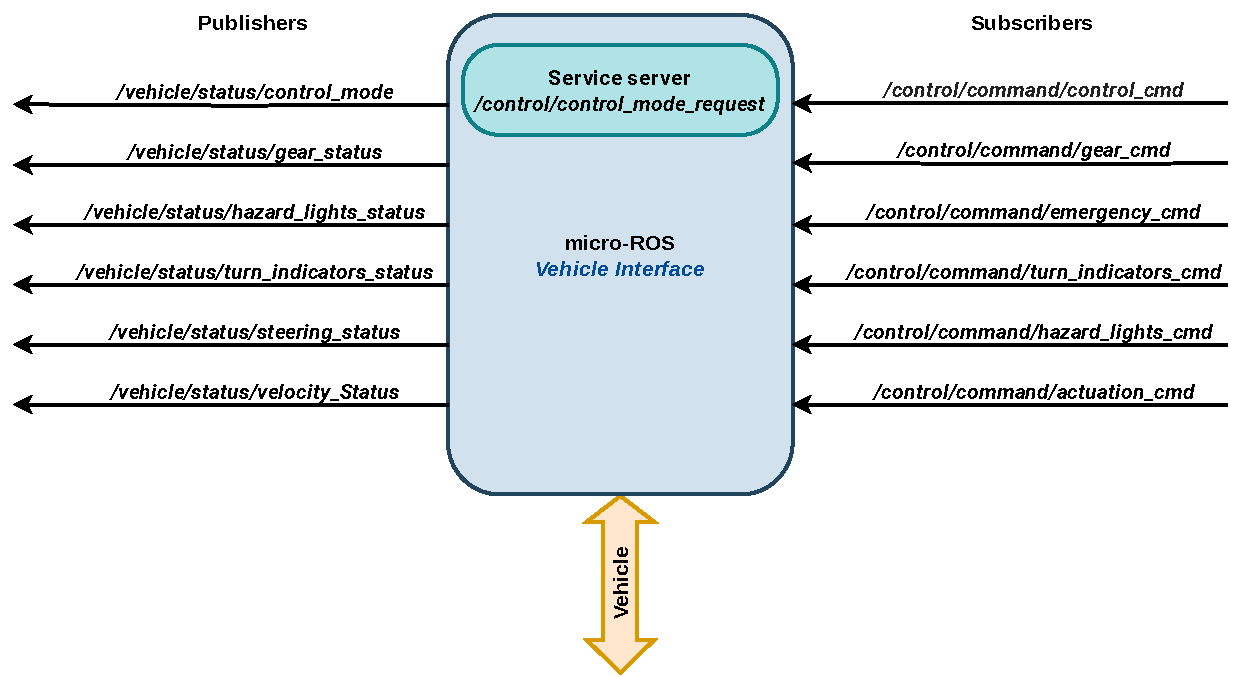
\includegraphics[width=0.75\linewidth]{img/vehicle_interface-topics}
	\caption{Diagrama de tópicos da \textit{vehicle interface}.}
	\label{fig:vehicleinterface-topics}
\end{figure}

\subsection{Requisitos}

\subsubsection*{Requisitos funcionais}
	
	\begin{itemize}
		\item Comunicação com o Autoware;
		\item Controle da aceleração, frenagem e direção do veículo;
		\item Controle dos faróis e luzes de sinalização (seta) do veículo;
		\item Teleoperação do veículo por um \textit{joystick} em  \textit{hardware};
		\item Troca do modo de operação por meio da \textit{switch} do \textit{joystick};
		\item Subscrição por meio do micro-ROS em todos os tópicos necessários do Autoware;
		\item Publicação a partir micro-ROS em todos os tópicos necessários do Autoware;
		\item Comunicação a partir micro-ROS em todos os serviços necessários do Autoware.
		
	\end{itemize}

\subsubsection*{Requisitos não funcionais}
	
	\begin{itemize}
		\item A \textit{vehicle interface} deve ser construída na forma de um pacote portável para outros microcontroladores STM32;
		\item O interfaceamento com o veículo deve ser intercambiável com diferentes configurações;
		\item Deve-se garantir sincronização de \textit{timestamp} entre o Autoware e o microcontrolador;
		\item O sistema embarcado deve abstraír o veículo como um sistema \textit{Drive-By-Wire} (DBW) para o Autoware.
	\end{itemize}
	
\subsection{Componentes}

\subsubsection*{Placa de desenvolvimento NUCLEO-H753ZI}
	
	\begin{itemize}
		\item Microcontrolador STM32H753ZI;
		\item ARM Cortex-M7;
		\item 1 MB RAM;
		\item 2 MB Flash;
		\item \textit{Clock} máximo de 480 MHz;
		\item DMA;
		\item Comunicação:
		\begin{itemize}
			\item UART/USART;
			\item Ethernet;
			\item USB.
		\end{itemize}
		\item Custo: US\$ 27,00.
	\end{itemize}

\begin{figure}[!h]
	\centering
	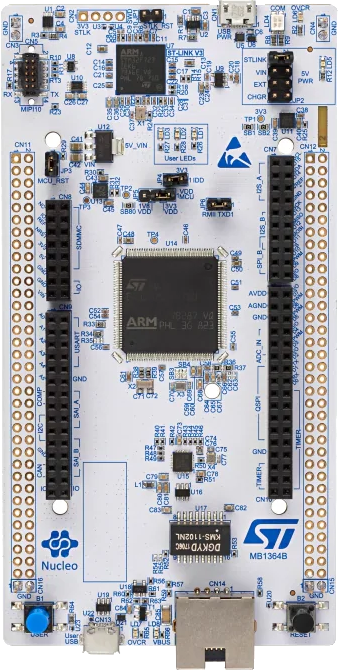
\includegraphics[width=0.25\linewidth]{img/nucleo}
	\caption{NUCLEO-753ZI.}
	\label{fig:nucleo}
\end{figure}

\clearpage

\subsubsection*{Joystick}
	
	\begin{itemize}
		\item Tensão de operação: 3V3 -- 5V;
		\item Saída analógica referente ao eixo $x$;
		\item Saída analógica referente ao eixo $y$;
		\item Saída digital referente ao eixo $z$;
		\item Custo: R\$ 10,00.
	\end{itemize}



\begin{figure}[!h]
\centering
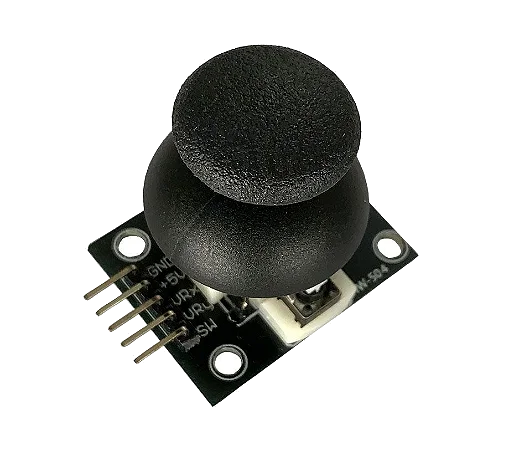
\includegraphics[width=0.3\linewidth]{img/joystick}
\caption{Joystick 2 eixos.}
\label{fig:joystick}
\end{figure}

\subsubsection*{Estação de trabalho}

\begin{itemize}
	\item Ubuntu 22.04 LTS;
	\item CPU Intel Core I7 5960X;
	\item 4x Memória RAM DDR4 8 GB;
	\item 2x GPU NVIDIA GEFORCE GTX TITAN X 12 GB;
	\item Custo: R\$ 10000,00.
\end{itemize}

\subsubsection*{Módulo FTDI}

\begin{itemize}
	\item Tensão de operação: 3V3 -- 5V;
	\item Circuito integrado: FT232RL;
	\item \textit{Baudrate} mínima: 183,1 bps;
	\item \textit{Baudrate} máxima: 3 Mbps;
	\item Custo: R\$ 20,00.
\end{itemize}

\clearpage

\subsection{Arquitetura}

A arquitetura HIL é baseada no uso de dois sistemas, um computador, executando o CARLA e o Autoware, e um sistema embarcado executando o FreeRTOS. A \autoref{fig:highLevelblock_diagram} mostra os blocos presentes em cada sistema e como eles se comunicam. Observa-se que o CARLA não recebe dadod diretamente do Autoware, e que existem duas linhas comunicação \textit{full-duplex}, entre o Autoware e a tarefa microAutoware, e entre o simulador e a tarefa TaskControle.

\begin{figure}[H]
	\centering
	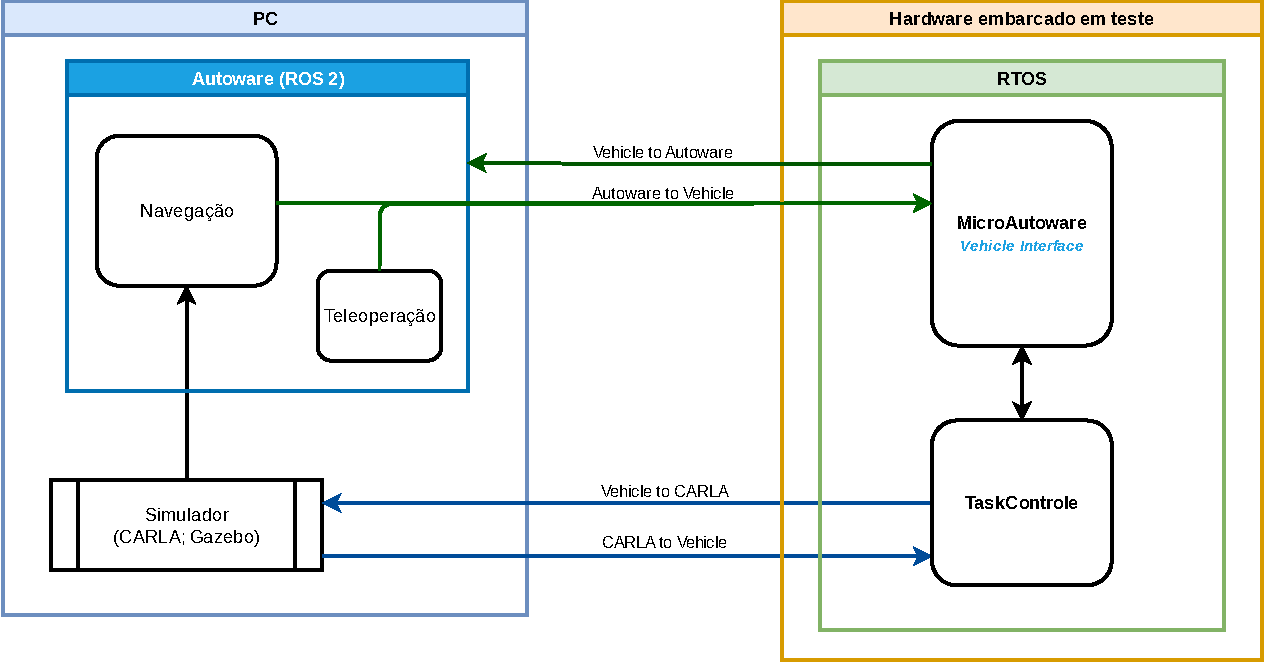
\includegraphics[width=0.7\linewidth]{img/highLevelblock_diagram.pdf}
	\caption{Diagrama de blocos em alto nível da arquitetura HIL.}
	\label{fig:highLevelblock_diagram}
\end{figure}

Especificando como a comunicação é feita, cada linha de comunicação é dada por uma porta de comunicação serial assíncrona (UART), sendo uma responsável pela comunicação com o Autoware, utilizando o agente do micro-ROS para o interfaceamento Serial-ROS, enquanto a outra se comunica com o simulador, por meio do pacote Carla-Serial-Bridge\footnote{Disponível em: \href{https://github.com/LMA-FEM-UNICAMP/carla_serial_bridge}{github.com/LMA-FEM-UNICAMP/carla\_serial\_bridge}}. A recepção e transmissão via UART é feita utilizando DMA, de forma a preservar o CPU e reduzir o tempo dentro da rotina de interrupção, sendo utilizado um módulo DMA para cada UART para evitar sobrecarga. Adicionalmente, para leitura do \textit{joystick} são utilizados duas entradas analógicas e uma entrada digital, que é atrelada à um canal de interrupções externas (EXTI).

\begin{figure}[H]
	\centering
	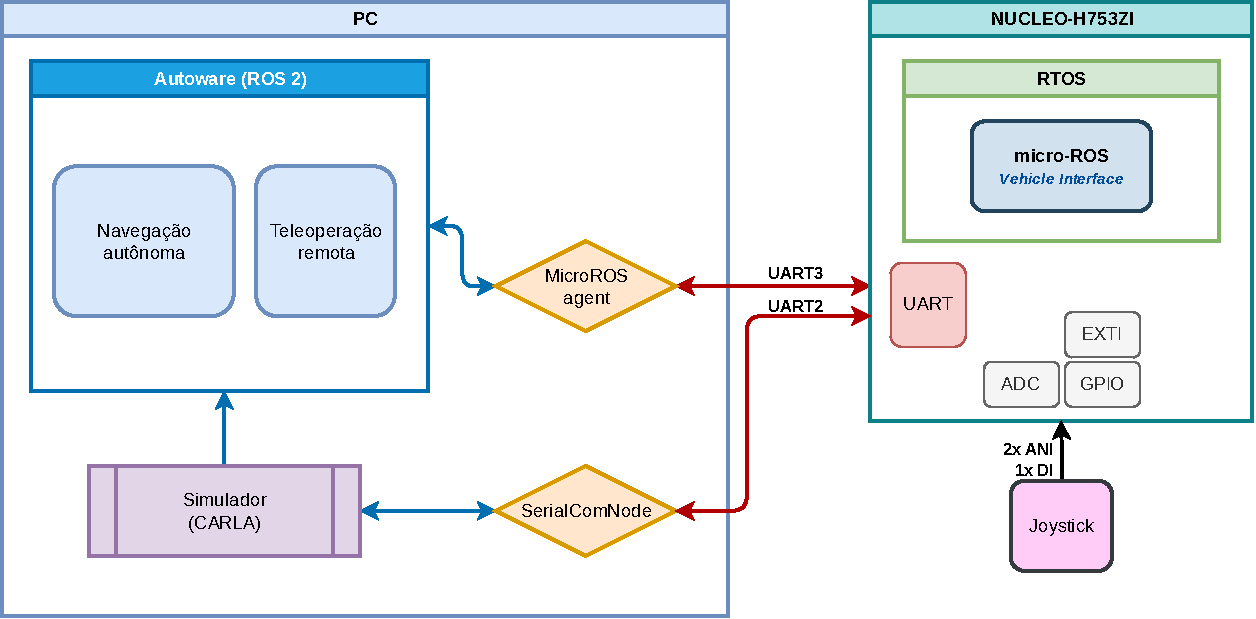
\includegraphics[width=0.7\linewidth]{img/block_diagram.pdf}
	\caption{Diagrama de blocos do sistema embarcado.}
	\label{fig:blockdiagram}
\end{figure}

A ligação física se dá como mostrado no esquemático da \autoref{fig:esquematico}, onde a alimentação do circuito é feita por meio da porta USB conectada ao ST-LINK. Um detalhe importante de montagem é que o pino de alimentação 3,3 V do módulo FTDI não foi conectado à placa NUCLEO, com intuito de evitar correntes parasitas no circuito de alimentação devido a desparidade de referência causada pelos conversores da NUCLEO e do FTDI. A montagem física é mostrada na \autoref{fig:montagem}.

\begin{figure}[H]
	\centering
	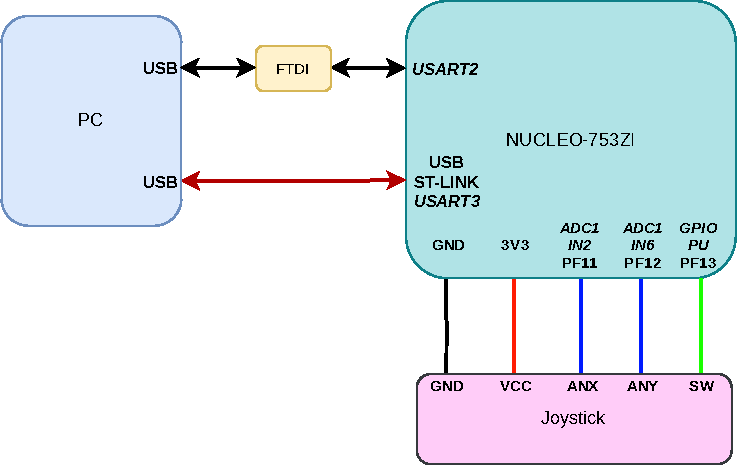
\includegraphics[width=0.55\linewidth]{img/esquematico.pdf}
	\caption{Esquemático de ligações elétricas.}
	\label{fig:esquematico}
\end{figure}

\begin{figure}[H]
	\centering
	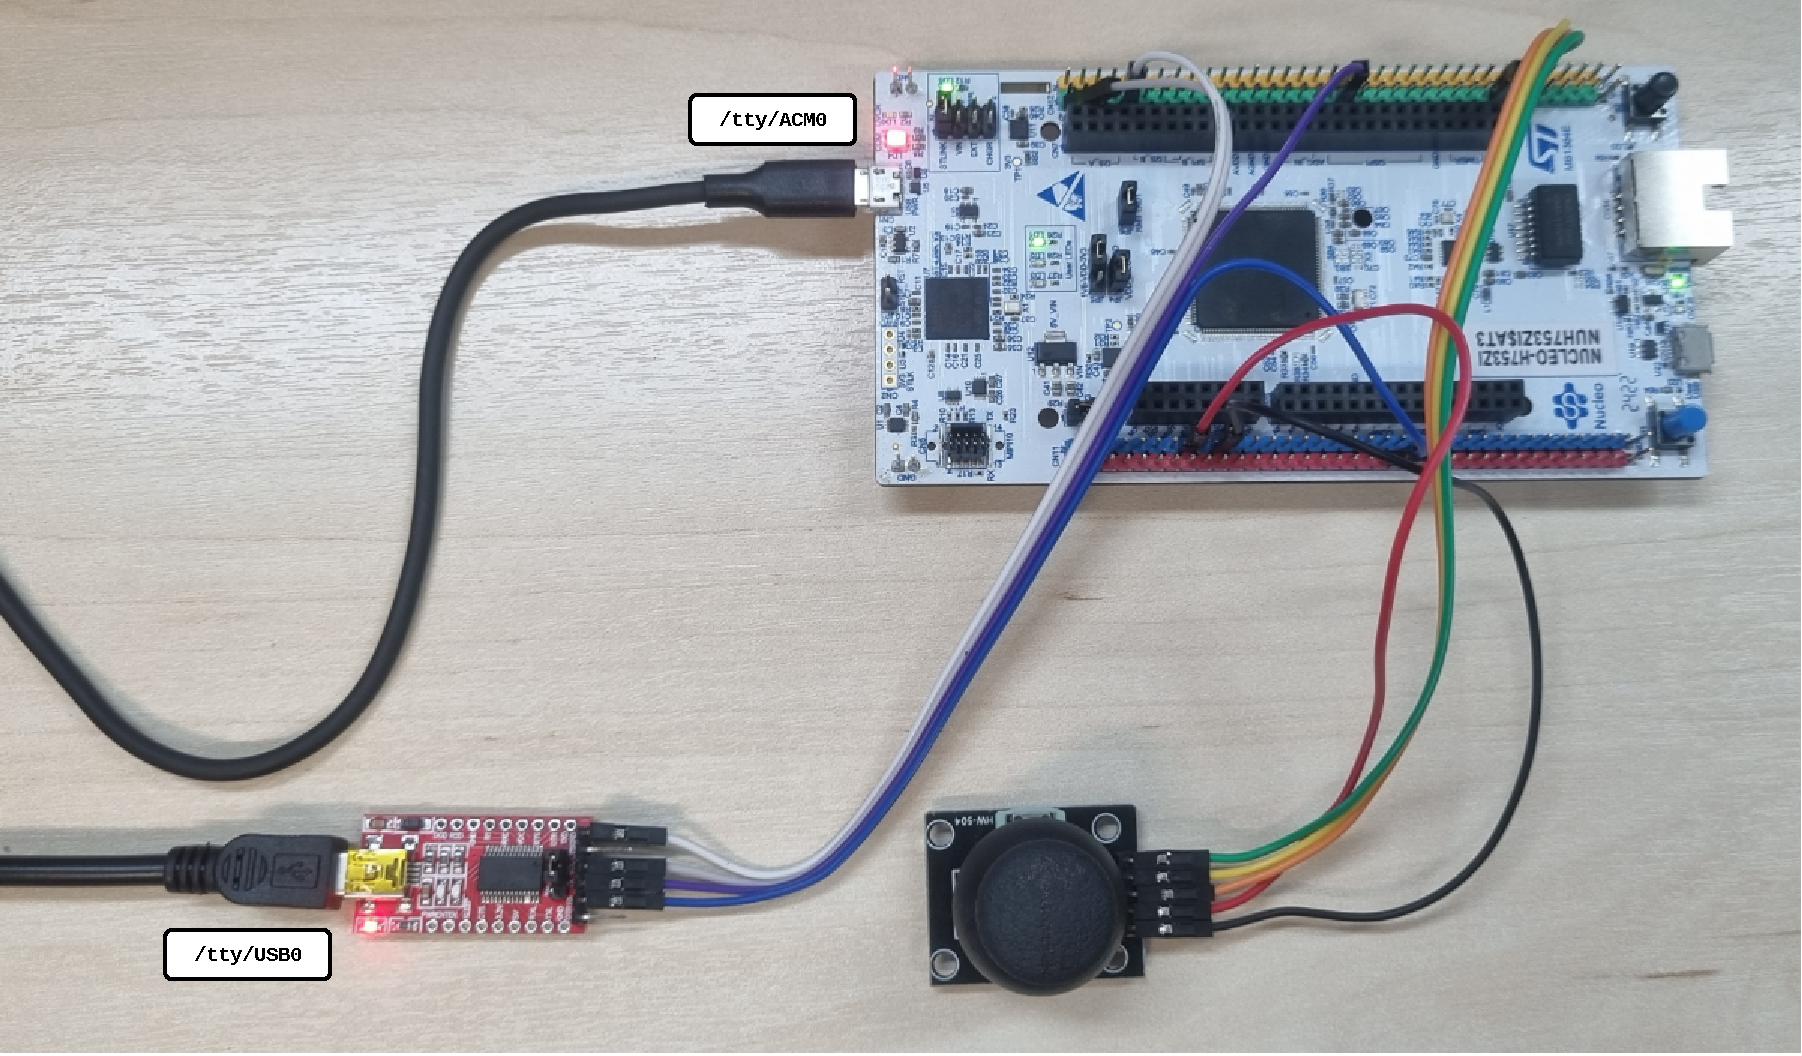
\includegraphics[width=0.7\linewidth]{img/montagem.pdf}
	\caption{Montagem do circuito.}
	\label{fig:montagem}
\end{figure}

\subsubsection*{Periféricos necessários}

\begin{itemize}
	\item \textit{Direct Memory Access}
	
	\item UART
	
	\item ADC
	
	\item GPIO
	
	\item EXTI
	
	
	
\end{itemize}


\clearpage

\subsection{Método de desenvolvimento}

Para realização das atividades necessárias para o desenvolvimento do projeto, foi selecionado o método V, onde, como mostrado na \autoref{fig:modelo-v}, as tarefas de criação são feitas em paralelo com as de validação, logo, permite a entrega final de forma confiável e sem a necessidad de re-manufaturar grandes módulos.

\begin{figure}[H]
	\centering
	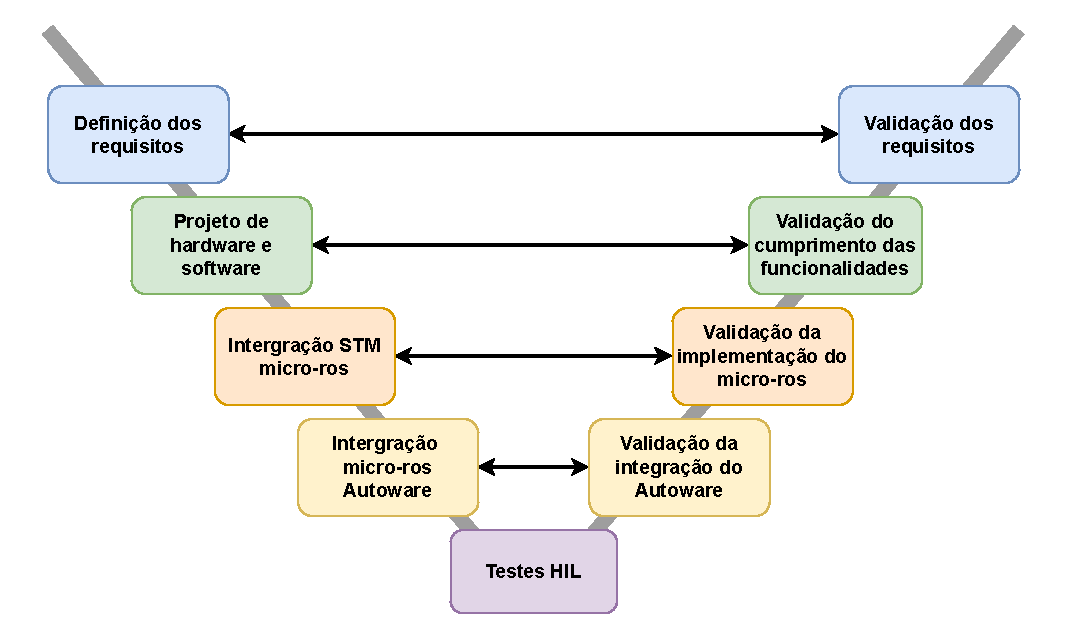
\includegraphics[width=0.75\linewidth]{img/modelo-v}
	\caption{Modelo de execução das atividades do projeto.}
	\label{fig:modelo-v}
\end{figure}

O projeto teve sua realização em um horizonte de 9 semanas, como mostrado na \autoref{tab:crono}, sendo realizadas entregas parciais nas semanas 2, 4, 7 e 9.

\begin{table}[H]
	\centering
	\small{
		\begin{tabular}{|c|c|c|c|c|c|c|c|c|c|}
			\hline
			\textbf{Atividade/Semana} & 1 & \textbf{2} & 3 & \textbf{4} & 5 & 6 & \textbf{7} & 8 & \textbf{9} \\
			\hline
			Proposta do projeto  & \cellcolor{unifeiblue} &  &  &  &  &  &  &  &  \\
			\hline
			Projeto de \textit{hardware} e \textit{software}  &  & \cellcolor{unifeiblue} & \cellcolor{unifeiblue} &  &  &  &  &  &  \\
			\hline
			Integração do STM com o micro-ROS  &  & \cellcolor{unifeiblue} &  &  &  &  &  &  &  \\
			\hline
			Integração do micro-ROS com o Autoware  &  &  & \cellcolor{unifeiblue} & \cellcolor{unifeiblue} & \cellcolor{unifeiblue} &  &  &  &  \\
			\hline
			Implementação das tarefas do sistema embarcado  &  &  &  & \cellcolor{unifeiblue} & \cellcolor{unifeiblue} & \cellcolor{unifeiblue} & \cellcolor{unifeiblue} &  &  \\
			\hline
			Construção do ambiente de testes  &  &  &  &  & \cellcolor{unifeiblue} & \cellcolor{unifeiblue} & \cellcolor{unifeiblue} &  &  \\
			\hline
			Realização dos testes  &  &  &  &  &  &  & \cellcolor{unifeiblue} & \cellcolor{unifeiblue} & \cellcolor{unifeiblue} \\
			\hline
			Escrita do relatório  &   & \cellcolor{unifeiblue} & \cellcolor{unifeiblue} & \cellcolor{unifeiblue} & \cellcolor{unifeiblue} & \cellcolor{unifeiblue} & \cellcolor{unifeiblue} & \cellcolor{unifeiblue} & \cellcolor{unifeiblue} \\
			\hline
		\end{tabular}
	}
	\caption{Cronograma de atividades.}
	\label{tab:crono}
\end{table}

\begin{itemize}
	\small
	\item \textbf{Semana 2:} Apresentação Etapa 1
	\item \textbf{Semana 4:} Apresentação Etapa 2
	\item \textbf{Semana 7:} Apresentação Etapa 3
	\item \textbf{Semana 9:} Apresentação Final
\end{itemize}

\clearpage

\subsection{Projeto de \textit{software}}

\subsubsection*{Estados do sistema}

O sistema pode se encontrar em três estados durante seu funcionamento: \texttt{AUTOWARE}, \texttt{MANUAL} ou \texttt{EMERGÊNCIA}, sendo o primeiro escolhido na inicialização. No primeiro, o veículo é conduzido pelos comandos do Autoware, e caso seja solicitado pelo Autoware ou pelo botão do \textit{joystick}, ou ainda se houver perda da \textit{deadline} de recebimento dos comandos do Autoware, o estado do sistema se altera para \texttt{MANUAL}. Neste segundo modo, o veículo é comandado pelo \textit{joystick}, podendo voltar à ser autonomo por comandos do próprio controle ou do Autoware. Para os dois estados iniciais, caso haja a perda da janela de tempo de recebimento dos sinais dosimulador, o sistema entra em modo \texttt{EMERGÊNCIA}, onde o veículo efetua uma parada de emergência. Caso a comunicação com o CARLA seja restaurada, o sistema retorna ao estado \texttt{MANUAL}.

\begin{figure}[H]
	\centering
	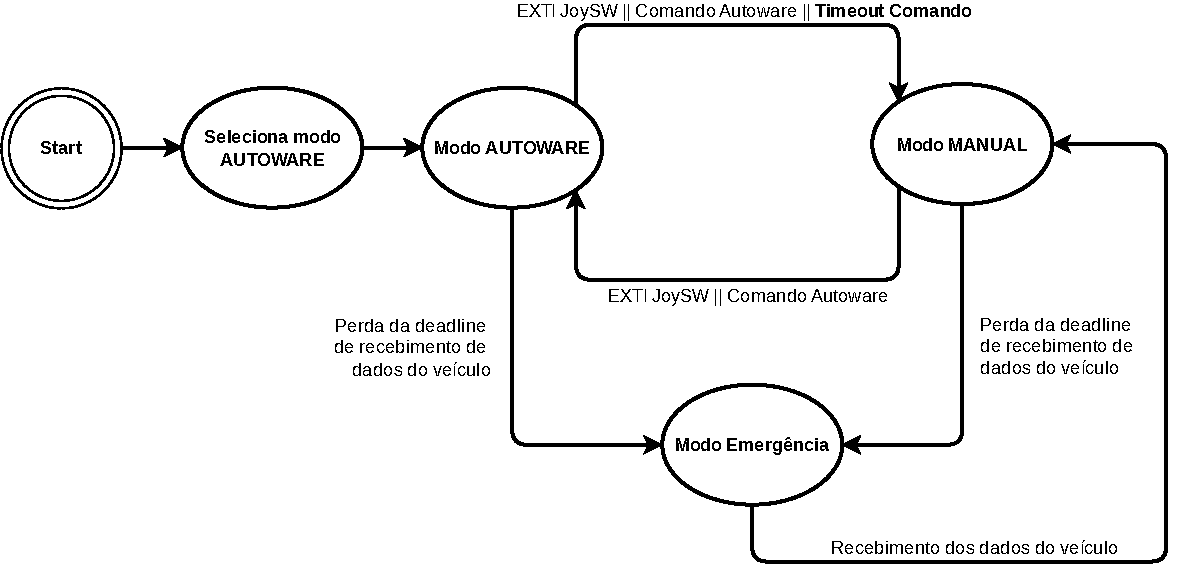
\includegraphics[width = 0.75\textwidth]{img/maquinadeestados}
	\caption{Máquina de estados do sistema.}
	\label{fig:maquinadeestados}
\end{figure}

\subsubsection*{Protocolo de comunicação serial}

A comunicação serial entre o sistema embarcado e o simulador é realizada por meio de um protocolo implementado via máquina de estados, onde a \autoref{fig:smuccarla} representa o envio de dados do microcontrolador para o CARLA, enquanto a \autoref{fig:sm_carla_uc} o caminho contrário.

\begin{enumerate}
	\item CARLA $\longrightarrow$ RTOS (\texttt{USART3})
	\begin{itemize}
		\item Informações:
		\begin{itemize}
			\item Velocidade longitudinal do veículo -- \texttt{float fLongSpeed;}
			\item Velocidade lateral do veículo -- \texttt{float fLatSpeed;}
			\item Taxa de guinada do veículo (velocidade angular no eixo $z$) -- \texttt{float fHeadingRate;}
			\item Ângulo de esterçamento da roda virtual -- \texttt{float fSteeringStatus;}		
		\end{itemize}
		\item Padrão da mensagem: \textbf{\#A}\texttt{\%c\%c\%c\%c}\textbf{B}\texttt{\%c\%c\%c\%c}\textbf{C}\texttt{\%c\%c\%c\%c}\textbf{D}\texttt{\%c\%c\%c\%c}\textbf{\$}
		\item Tamanho da mensagem: 22 bytes;
		\item Envia uma \textit{ThreadFlag} ao receber a mensagem inteira.
		
	\end{itemize}
	\item RTOS $\longrightarrow$ CARLA (\texttt{USART2})
	\begin{itemize}
		\item Informações:
		\begin{itemize}
			\item Ângulo de esterçamento desejado do volante -- \texttt{float fSteeringAngle;}
			\item Velocidade de esterçamento do volante -- \texttt{float fSteeringVelocity;}
			\item Velocidade linear desejada para o veículo -- \texttt{float fSpeed;}
			\item Aceleração linear desejada para o veículo -- \texttt{float fAcceleration;}
			\item \textit{Jerk} linear desejada para o veículo -- \texttt{float fJerk;}	
			\item Modo de controle -- \texttt{unsigned char ucControlMode;}		
		\end{itemize}
		\item Padrão da mensagem: \textbf{\#S}\texttt{\%c\%c\%c\%c}\textbf{W}\texttt{\%c\%c\%c\%c}\textbf{V}\texttt{\%c\%c\%c\%c}\textbf{A}\texttt{\%c\%c\%c\%c}\textbf{J}\texttt{\%c\%c\%c\%c}\textbf{M}\texttt{\%c}\textbf{\$}
		\item Tamanho da mensagem: 30 bytes.
		
	\end{itemize}
\end{enumerate}


% TODO: \usepackage{graphicx} required
\begin{figure}[H]
	\centering
	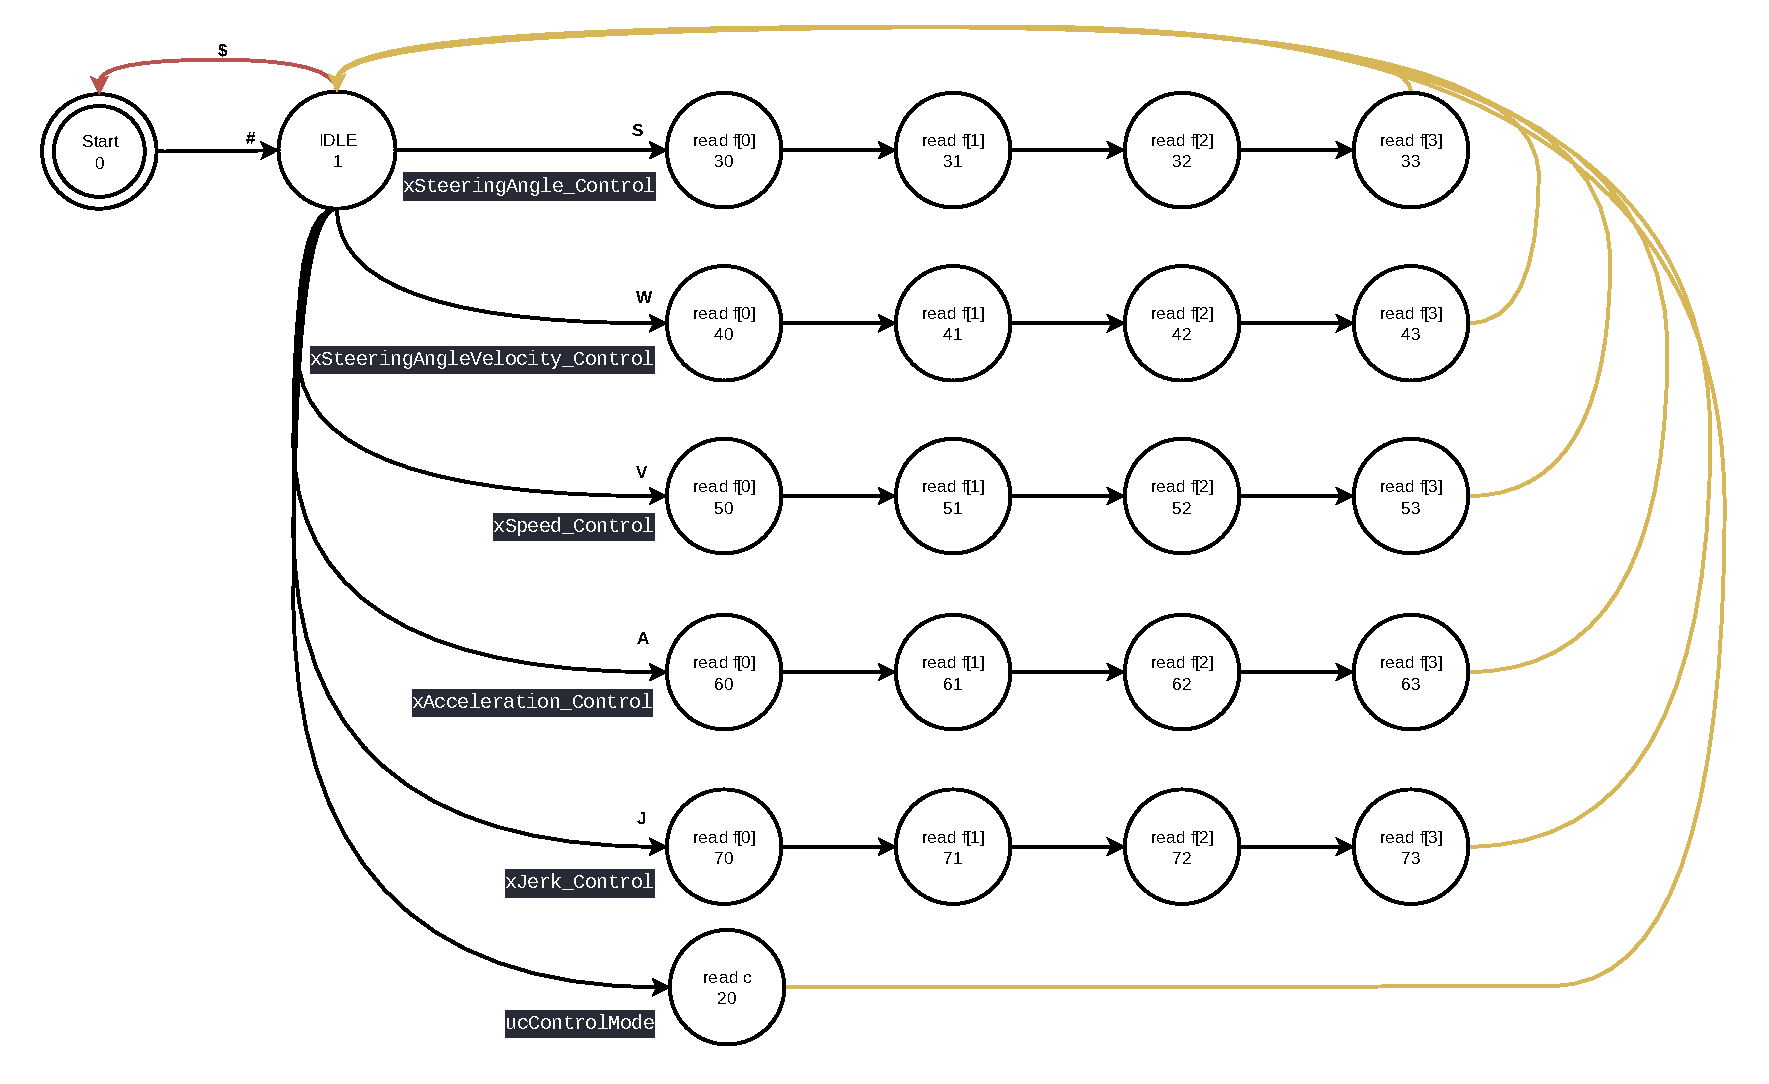
\includegraphics[width=0.8\linewidth]{img/sm_uc_2_carla}
	\caption{Máquina de estados da comunicação serial do RTOS para o CARLA.}
	\label{fig:smuccarla}
\end{figure}


% TODO: \usepackage{graphicx} required
\begin{figure}[H]
\centering
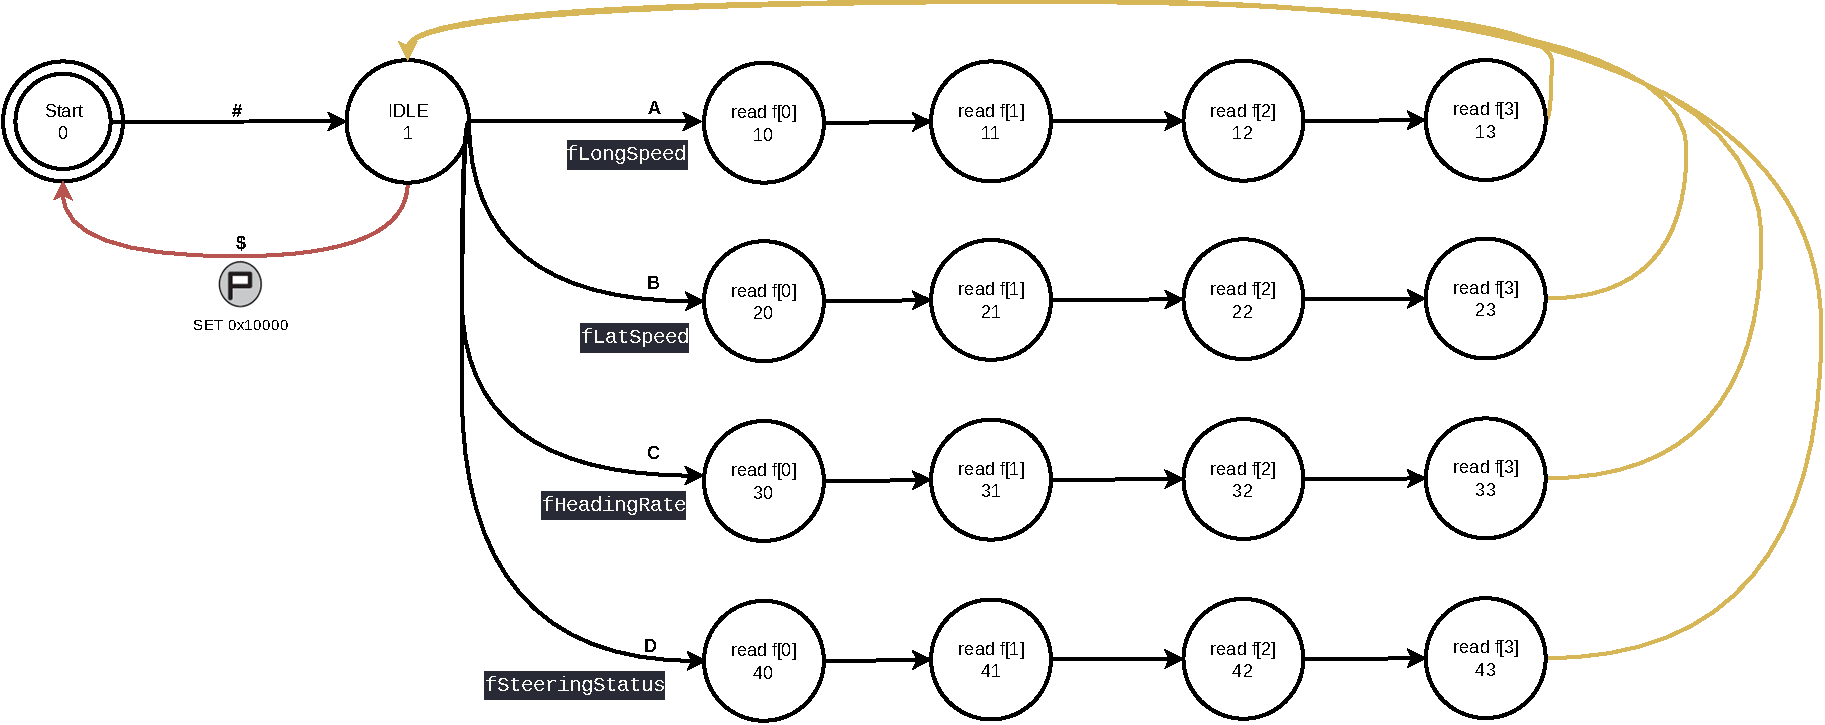
\includegraphics[width=0.8\linewidth]{img/sm_carla_2_uc}
\caption{Máquina de estados da comunicação serial do CARLA para o RTOS.}
\label{fig:sm_carla_uc}
\end{figure}



\subsubsection*{Tarefas}

O sistema embarcado de tempo real foi estruturado por meio de duas tarefas: microAutoware, responsável pela comunicação com o Autoware e TaskControle, incubida pelo controle do veículo. Essas tarefas se comunicam por meio de variáveis globais protegidas por MUTEX e são sincronizadas por \textit{ThreadFlags}. São empregadas também interrupções para comunicação serial e leitura do botão do \textit{joystick}, como representado no diagrama da \autoref{fig:systemdiagram}.

\begin{figure}[H]
	\centering
	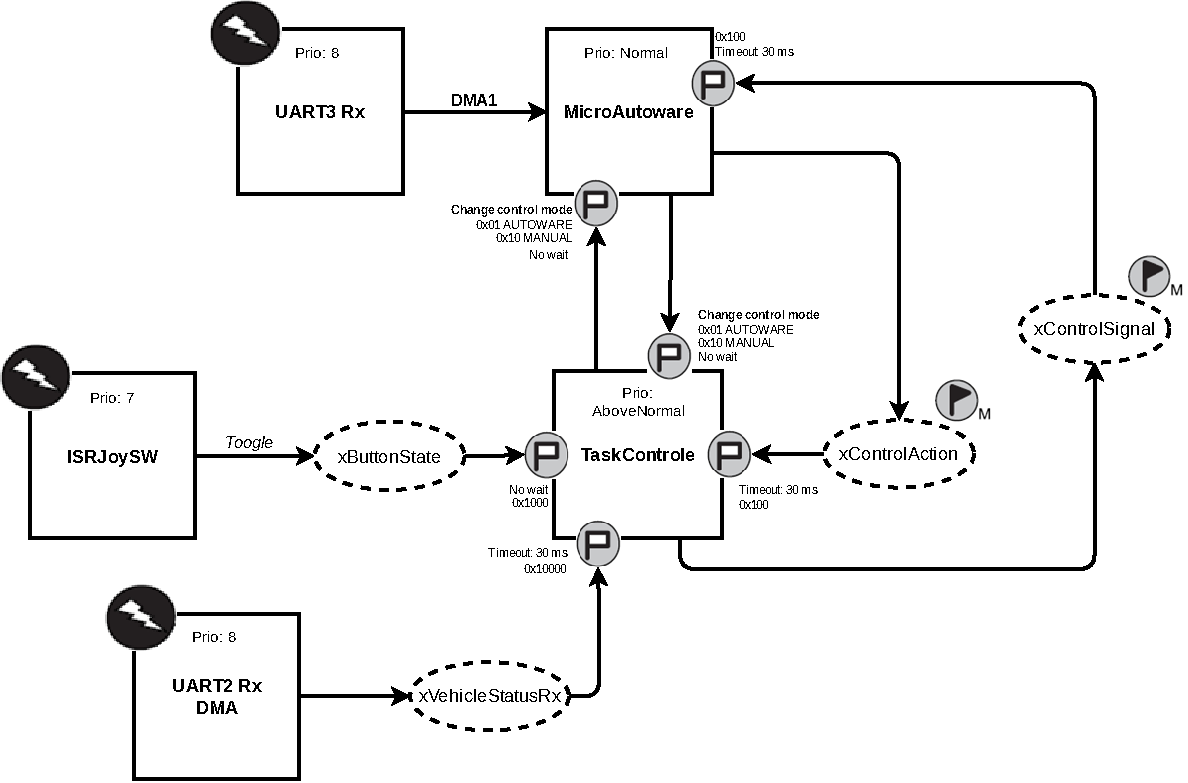
\includegraphics[width = \textwidth]{img/system_diagram}
	\caption{Diagrama do sistema embarcado.}
	\label{fig:systemdiagram}
\end{figure}

\noindent MicroAutoware

\begin{table}[H]
	\centering
	\begin{tabular}{c|p{11.5cm}}
		\textbf{Nome} & MicroAutoware \\
		\hline
		\textbf{Prioridade}& Normal \\
		\hline
		\textbf{Tamanho da stack} & 3500 kB \\
		\hline
		\textbf{Detalhes} & Realiza a leitura dos \textit{subscribers} do Autoware executando o executor por um certo tempo, envia das informações de controle e modo de operação para a TaskControle, e ao receber as informações de controle da TaskControle, às escreve nos \textit{publishers} do Autoware.\\
	\end{tabular}
	\caption{Especificaçõe da tarefa MicroAutoware.}
	\label{tab:microautoware}
\end{table}

\begin{figure}[H]
	\centering
	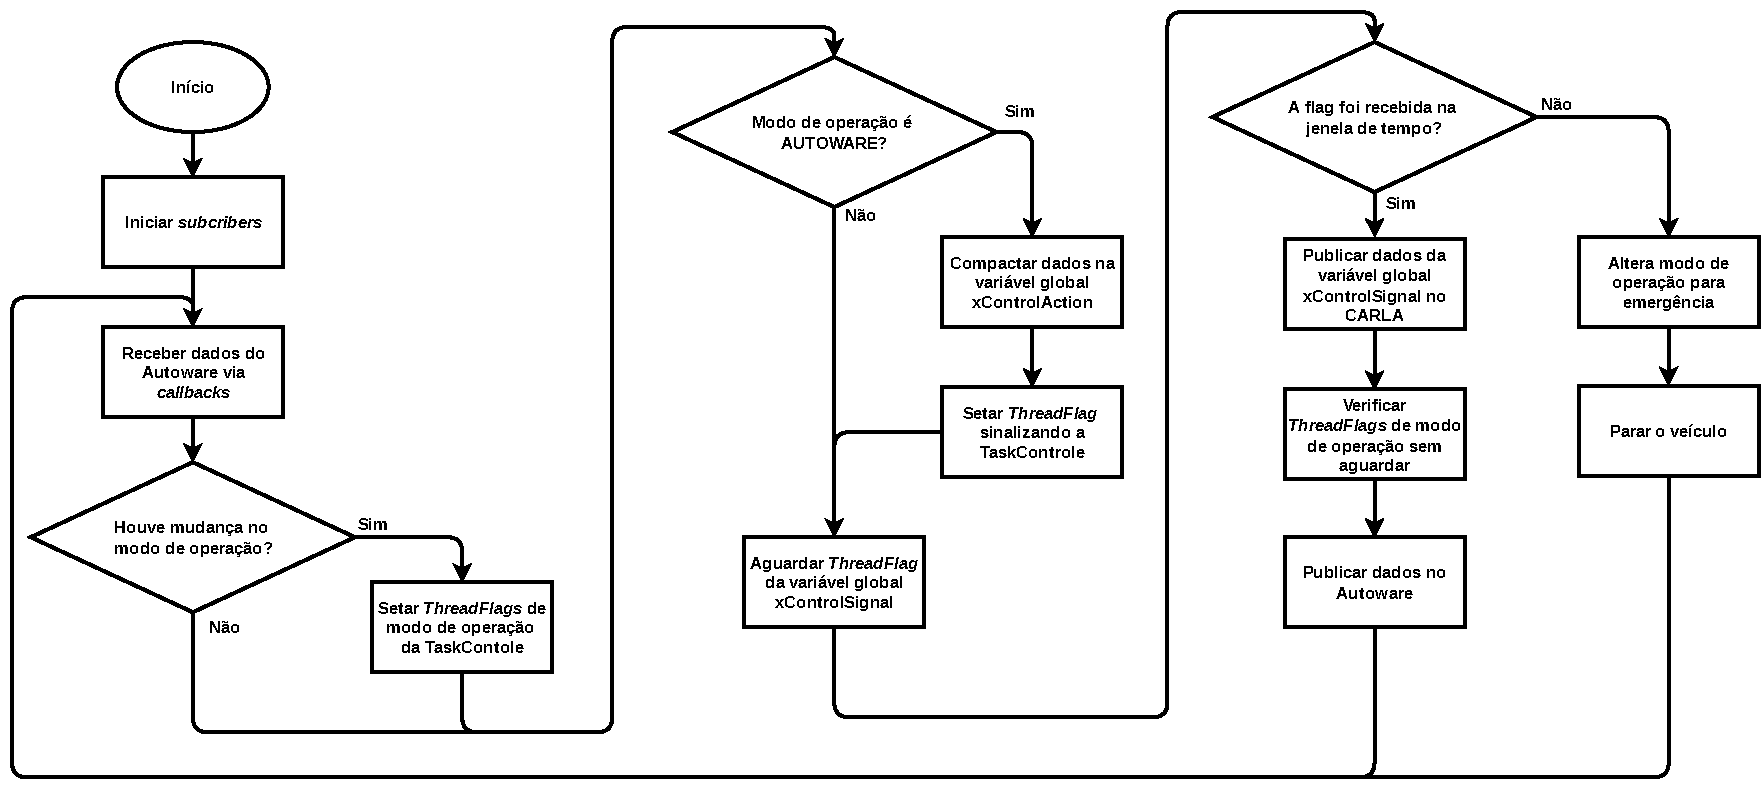
\includegraphics[width = \textwidth]{img/fluxograma_microautoware}
	\caption{Fluxograma da tarefa MicroAutoware.}
	\label{fig:fluxograma_microautoware}
\end{figure}

\noindent TaskControle

\begin{table}[H]
	\centering
	\begin{tabular}{c|p{11.5cm}}
	\textbf{Nome} & TaskControle \\
	\hline
	\textbf{Prioridade}& AboveNormal \\
	\hline
	\textbf{Tamanho da stack} & 500 kB \\
	\hline
	\textbf{Detalhes} & Realiza o controle do veículo utilizando a referência dada pelo \textit{joystick} ou pelo Autoware, dado o modo de operação, podendo ser MANUAL ou AUTOWARE, respectivamente. A alteração do modo é feita por \textit{ThreadFlag}, gerada por ISR ou pelo Autoware. Em caso do modo de operação AUTOWARE, os sinais de controle são recebidos por variável global e sincronizados por \textit{ThreadFlag}, com tempo de 30 ms, onde caso não receba, entra em algum modo de segurança. Em caso de operação MANUAL,  o \textit{joystick} é lido por DMA, aguardando 60 ms antes de cada leitura,  convertendo os valores analógicos em sinais de controle, onde também caso haja algum erro, o modo de emergência é acionado. O sinal de controle é enviado para o MicroAutoware por uma variável global e sincronizado por \textit{ThreadFlag}. 
	\end{tabular}
	\caption{Especificaçõe da tarefa TaskControle.}
	\label{tab:taskcontrole}
\end{table}

\begin{figure}[H]
	\centering
	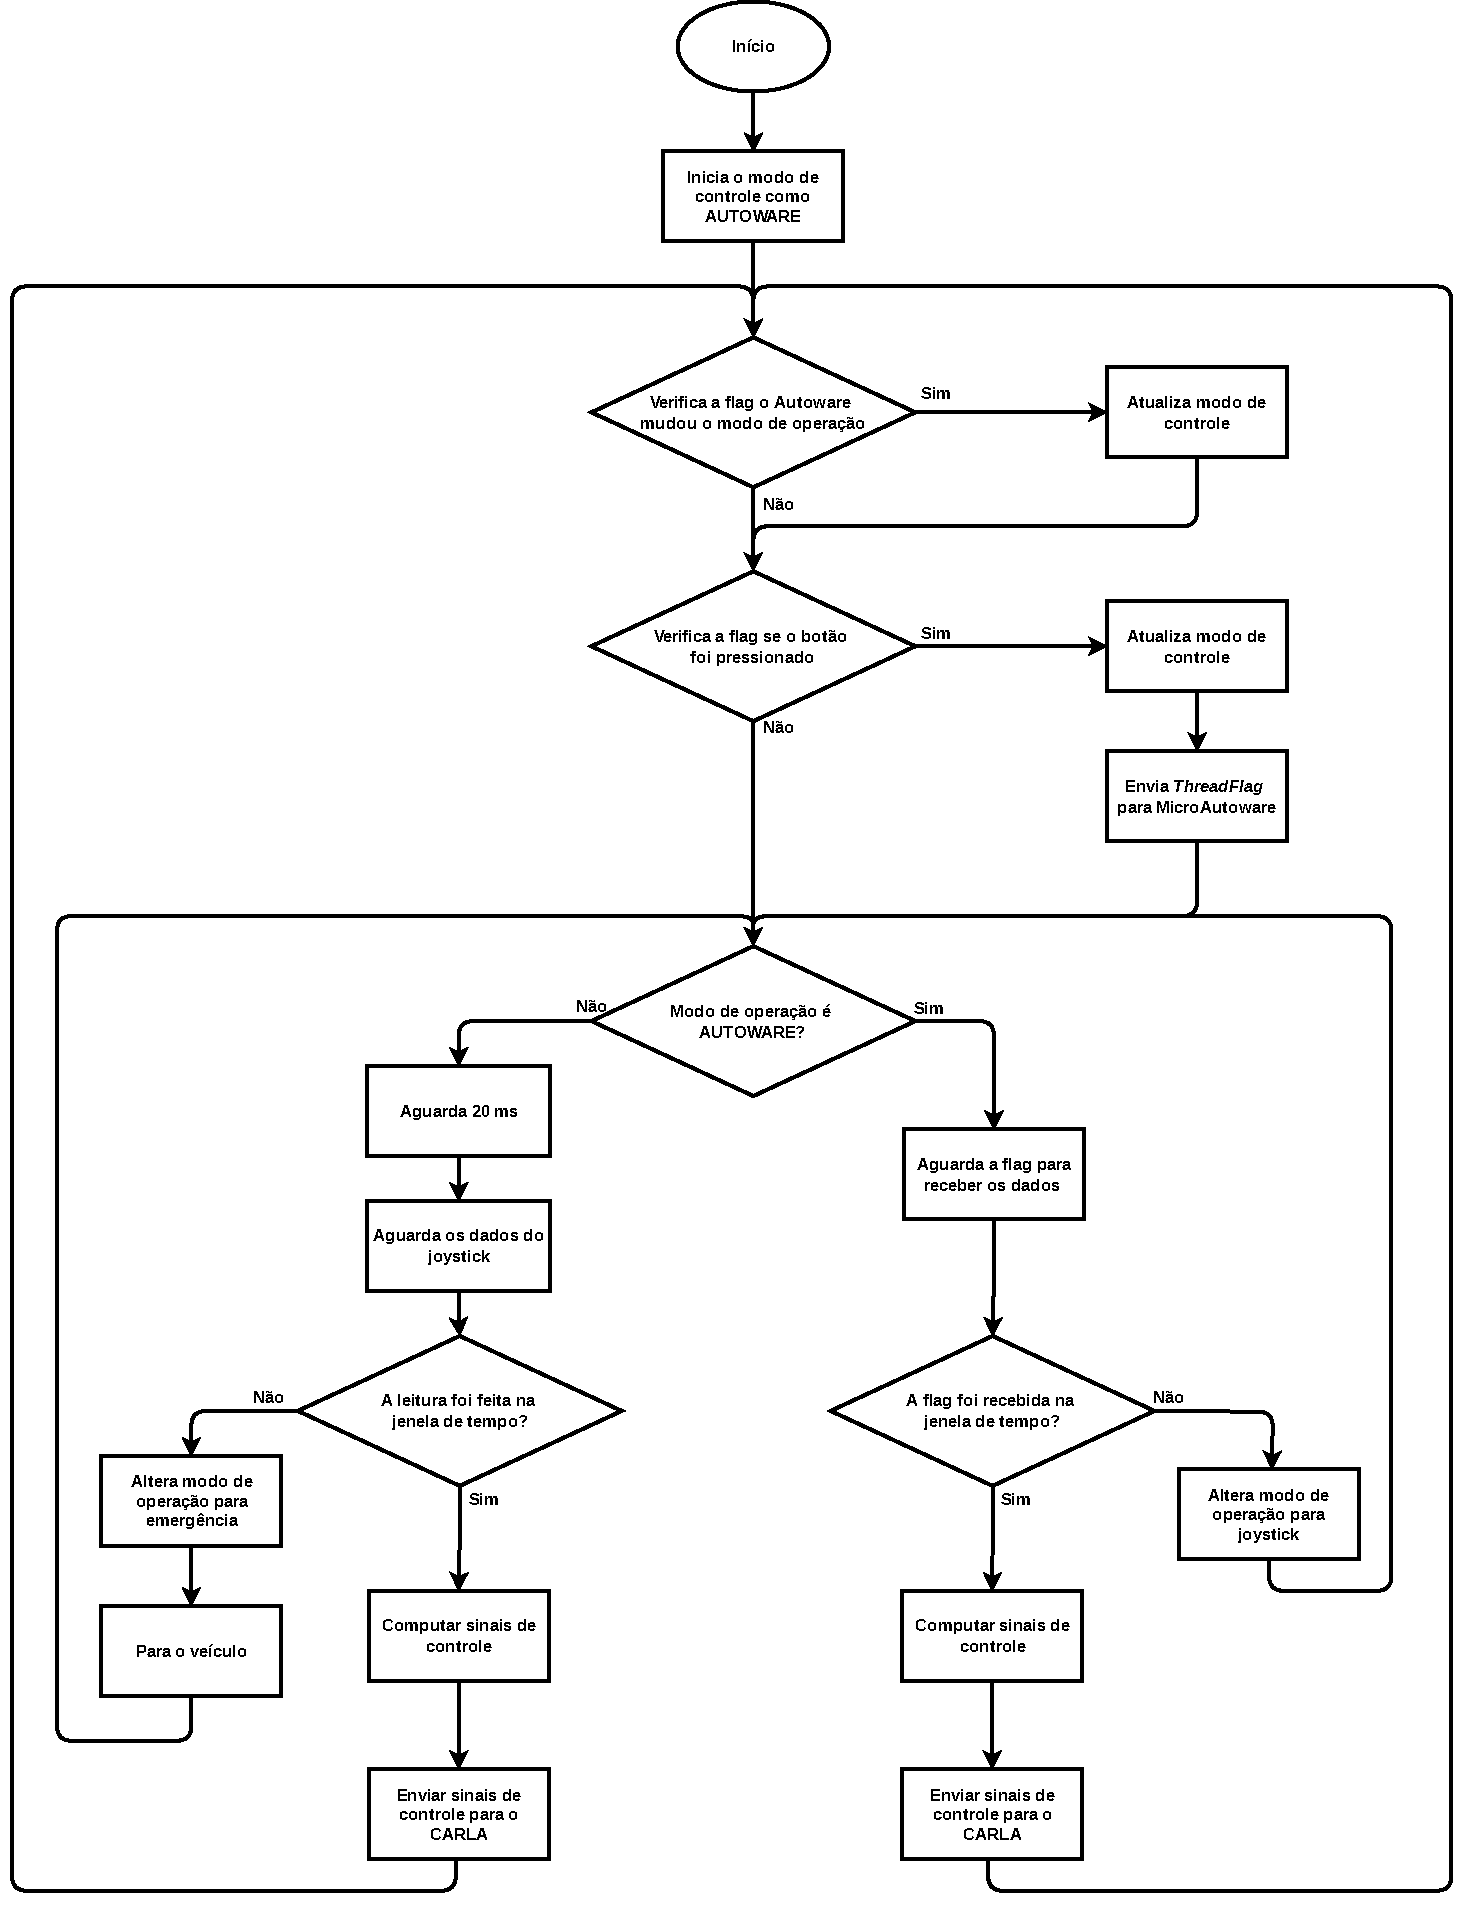
\includegraphics[height= 1\textheight]{img/fluxograma_taskcontrole}
	\caption{Fluxograma da tarefa TaskControle.}
	\label{fig:fluxograma_taskcontrole}
\end{figure}

\noindent Interrupções

\begin{figure}[H]
	\centering
	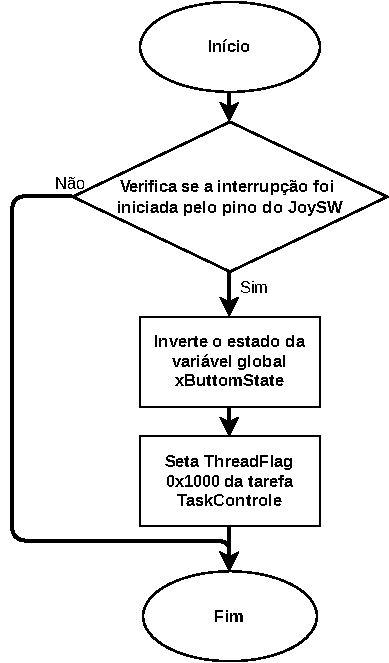
\includegraphics[height= 0.35\textheight]{img/fluxograma_joysw}
	\caption{Fluxograma da ISR JoySW.}
	\label{fig:fluxograma_joysw}
\end{figure}


\begin{figure}[H]
\centering
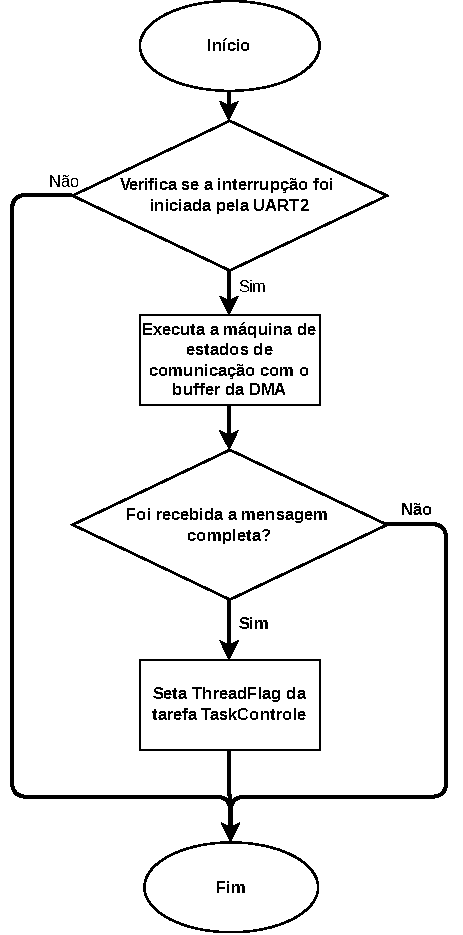
\includegraphics[height= 0.5\textheight]{img/fluxograma_uart2}
\caption{Fluxograma da ISR UART\_RxCpltCallback.}
\label{fig:fluxograma_uart2}
\end{figure}

\subsubsection*{Sinalização \texttt{xButtonState}}
	
	\begin{itemize}
		\item \textbf{Objeto:} \textit{ThreadFlag}
		\item \textbf{Flag:} 0x1000
		\item \textbf{Modo:} \textit{No wait}
		\item \textbf{Descrição:} Sinaliza ocorrência da interrupção do botão JoySW.
		
	\end{itemize}


\subsubsection*{Sinalização \texttt{xControlAction}}
	
	\begin{itemize}
		\item \textbf{Objeto:} \textit{ThreadFlag}
		\item \textbf{Flag:} 0x0100
		\item \textbf{Modo:} \textit{Timeout} 110 ms
		\item \textbf{Descrição:} Sinaliza o recebimento de dados pela variável global \texttt{xControlAction}.
		
	\end{itemize}	

\subsubsection*{Sinalização \texttt{xControlSignal}}
	
	\begin{itemize}
		\item \textbf{Objeto:} \textit{ThreadFlag}
		\item \textbf{Flag:} 0x0100
		\item \textbf{Modo:} \textit{No wait}
		\item \textbf{Descrição:} Sinaliza o recebimento de dados pela variável global \texttt{xControlSignal}.
		
	\end{itemize}	



\subsubsection*{Alteração do modo de condução por interrupção JoySW}
	
	\begin{itemize}
		\item \textbf{Objeto:} \textit{ThreadFlag}
		\item \textbf{Flags:}
		\begin{itemize}
			\item Modo de controle alterado para AUTOWARE: 0x01
			\item Modo de controle alterado para MANUAL: 0x10
			
		\end{itemize}
		\item \textbf{Modo:} \textit{No wait}
		\item \textbf{Descrição:} Realiza a sincronização do modo de operação da tarefa TaskControle para a MicroAutoware.
		
	\end{itemize}

\subsubsection*{Alteração do modo de condução pelo Autoware}
	
	\begin{itemize}
		\item \textbf{Objeto:} \textit{ThreadFlag}
		\item \textbf{Flags:}
		\begin{itemize}
			\item Modo de controle alterado para AUTOWARE: 0x01
			\item Modo de controle alterado para MANUAL: 0x10
			
		\end{itemize}
		\item \textbf{Modo:} \textit{No wait}
		\item \textbf{Descrição:} Realiza a sincronização do modo de operação da tarefa MicroAutoware para a TaskControle.
		
	\end{itemize}


\subsubsection*{Proteção de recursos}



\noindent {Variável global \texttt{xControlSignal}}
	
	\begin{itemize}
		\item Protegida por MUTEX.
		\begin{itemize}
			\item \texttt{MutexControlSignal}
			
		\end{itemize}
	\end{itemize}



\noindent {Variável global \texttt{xControlAction}}
	
	\begin{itemize}
		\item Protegida por MUTEX.
		\begin{itemize}
			\item \texttt{MutexControlAction}
			
		\end{itemize}
		
	\end{itemize}

\subsubsection*{Padronização de código ROS}

O ecossistema ROS possuí uma padronização de código própria, para identificação das suas entidades, como tópicos, nós e serviços. Dessa forma, essa padronização será adotada de forma excepcional para os atributos do micro-ROS, de acordo com o mostrado abaixo.
	
	\begin{itemize}
		\item Subscriber: \texttt{nome\_subscriber\_sub\_}
		\item Publisher: \texttt{nome\_subscriber\_pub\_}
		\item Service server: \texttt{nome\_subscriber\_server\_}
		\item Mensagem: \texttt{nome\_mensagem\_msg\_}
		\item Node: \texttt{nome\_do\_node}
		\item Callback: \texttt{nome\_do\_topico\_callback}
		
	\end{itemize}

\subsection{Periféricos}

\subsubsection*{Joystick}

\begin{enumerate}
	\item Eixos $x$ e $y$
	\begin{itemize}
		\item ADC de 16 bits \textit{multi-channel};
		\begin{itemize}
			\item Leitura contínua por DMA;
			\item Modo de \textit{clock} assíncrono dividido por 256;
			\item Tempo de amostragem de 387,5 ciclos;
			\item Interrupções desativadas para preservar a CPU.
			
		\end{itemize}				
	\end{itemize}
	
	\item Botão
	\begin{itemize}
		\item GPIO em modo \textit{pull-up};
		\item Interrupção EXTI.
		
	\end{itemize}

\end{enumerate}

\noindent \textit{Processamento de sinais}

Para conversão do valor discreto de leitura analógica obtido por meio do conversor analógico-digital (\textit{analogue-digital converter -- ADC}), foi realizada uma etapa de calibração, onde foram tomadas as medidas dos valores máximos, mínimos e de zero para os dois eixos do \textit{joystick}. Tomado esses valores, foi realizado o processo de linearização por partes, onde o valor discreto obtido, é mapeado no intervalo $(-1, 1)$, considerando uma banda morta $B$ ao redor do zero para evitar flutuação de zero e melhorar a usabilidade dos eixos de forma independente.

O a interpolação é realizada por meio de \eqref{eq:joy}, resultando nos gráficos mostrados nas Figuras~\ref{fig:plotjoyxaxis}~e~\ref{fig:plotjoyyaxis}, para o mapeamento nos eixos $x$ e $y$, respectivamente.

O eixo $x$ é alocado como a variável de esterçamento do volante, enquanto o eixo $y$ representa os sinais de acelerador e freio. Para valores positivos do eixo $y$, obtém-se a medida do acelerador no intervalo $(0,1)$, enquanto para valores negativos o freio é mapeado entre 0 e 1.

\begin{equation}\label{eq:joy}
	p(v) = \begin{dcases}
		0\vphantom{\frac{0}{0}}, &\text{se } - B \le v - V_0 \le B \\
		\frac{v - V_0 - B}{V_{max} - V_0 - B}, &\text{se } v > V_0 + B \\
		\frac{v - V_0 + B}{V_0 - V_{min} - B}, &\text{se } v < V_0 - B 
	\end{dcases}
\end{equation}

\begin{figure}[H]
	\centering
	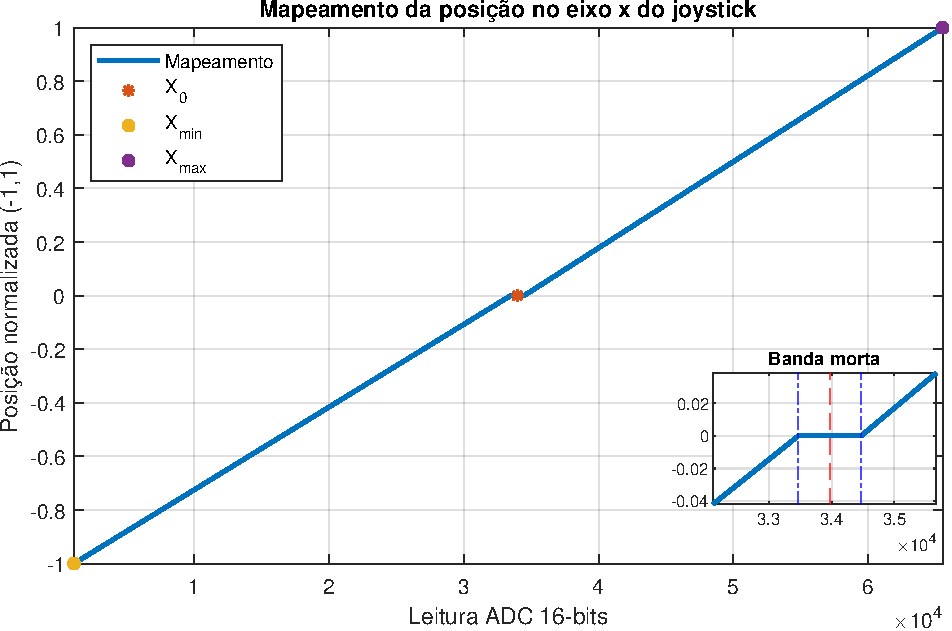
\includegraphics[width=0.75\linewidth]{img/plot_joy_x_axis.pdf}
	\caption{Mapeamento da posição no eixo $x$ normalizada do \textit{joystick} de acordo com a leitura analógia do ADC.}
	\label{fig:plotjoyxaxis}
\end{figure}


\begin{figure}[H]
\centering
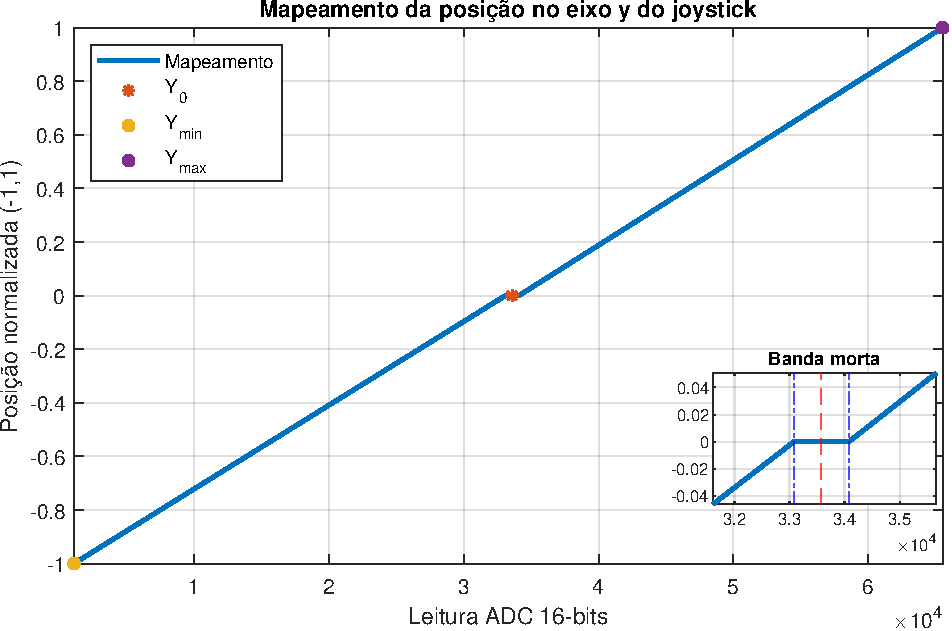
\includegraphics[width=0.75\linewidth]{img/plot_joy_y_axis.pdf}
\caption{Mapeamento da posição no eixo $y$ normalizada do \textit{joystick} de acordo com a leitura analógia do ADC.}
\label{fig:plotjoyyaxis}
\end{figure}

\clearpage

\subsubsection*{Comunicação serial -- UART}

	\begin{enumerate}
		\item UART2 -- Comunicação com o simulador.
		\begin{itemize}
			\item \textbf{\textit{Baudrate}:} 921600 bps
			\item \textbf{Modo de leitura:} DMA única;
			\item \textbf{Modo de escrita:} DMA única;
			\item \textbf{Interface física:} Módulo FTDI.	
		\end{itemize}
	
		\item UART3 -- Comunicação com o Autoware (micro-ROS \textit{agent}).
		\begin{itemize}
			\item \textbf{\textit{Baudrate}:} 921600 bps
			\item \textbf{Modo de leitura:} DMA circular;
			\item \textbf{Modo de escrita:} DMA única;
			\item \textbf{Interface física:} ST-LINK.		
		\end{itemize}	
	
	\end{enumerate}

\clearpage

\section{Manual de utilização}

\subsection{Inicialização}

\begin{enumerate}
	\item Conectar a placa ao computador;
	\item Conectar o módulo FTDI ao computador;
	\item Iniciar o agente micro-ROS;
	\item Iniciar o nó do ROS \texttt{carla\_serial\_bridge\_node};
	\item Iniciar o CARLA Simulator;
	\item Lançar o Carla-Autoware-Bridge no ROS;
	\item Lançar o Autoware em modo simulação.
\end{enumerate}

\subsection{Modo \texttt{AUTOWARE}}

\begin{enumerate}
	\item Passar uma velocidade limite pela interface do Autoware;
	\item Definir o ponto de objetivo no Autoware;
	\item Selecionar o modo de controle \texttt{AUTO};
	\item Caso o sistema esteja em modo \texttt{MANUAL}, pressionar o botão do \textit{joystick};
	\item Aguardar o veículo chegar ao destino.
\end{enumerate}

\subsection{Modo \texttt{MANUAL}}

\begin{enumerate}
	\item Caso o sistema esteja em modo \texttt{AUTOWARE}, pressionar o botão do \texttt{joystick};
	\item Mover o analógico do \textit{joystick} para frente para acelerar;
	\item Mover o analógico do \textit{joystick} para esquerda e direita para virar o volante;
	\item Mover o analógico do \textit{joystick} para trás para freiar.
\end{enumerate}

\clearpage


\section{Problemas identificados e não resolvidos}

\subsection*{Perda de resposta do serviço de troca de modo de controle}

O Autoware faz a utilização do serviço \texttt{/control/control\_mode\_request} para solicitar a \textit{vehicle interface} que faça a troca do modo de controle, realizando o engate do controle via Autoware ou remoção do mesmo. Esse tipo de comunicação ocorre da forma requisição--resposta, onde é feita a requisição de troca para o modo desejado e é respondido o resultado dessa troca (sucesso ou falha). 

Porém, constantemente ocorre a falha da resposta desse serviço, ocasionando o travamento do processo de transição de modo de controle. Após testes em diferentes máquinas e pesquisas em fóruns da comunidade, o problema ocorre provavelmente por alguma incompatibilidade do micro-ROS com a CycloneDDS, utilizada pelo Autoware, onde a resposta do servidor é perdida.


\subsection*{Perda de \textit{deadline} causada pela sobrecarga da estação de trabalho}

O sistema embarcado faz uso de um sistema operacional de tempo real, que entre suas premissas, trás o determinismo, onde seu comportamento é conhecido e constante. Já a estação de trabalho utilizada, faz uso de um sistema operacional de propósito geral, que não possuí garantias de determinismo. Dessa forma, quando ocorre a execução de algum processo que demanda alto poder computacional, outros processos acabam sendo interferidos, o que resulta no escopo do projeto, principalmente no aumento do período de envio de dados por parte do CARLA e Autoware.

Com isso, o aumento do tempo entre o recebimento de dados, em situações críticas faz com que ocorra a perda de \textit{deadlines} e o sistema embarcado execute alguma rotina de falha, como a mudança para direção manual ou modo de emergência. Para evitar a ocorrência de falsas falhas, a janela de tempo de recebimento de dados foi aumentada, e também foi realizada a prática de somente inicar o baixo nível uma vez que o alto nível já está funcional.


\subsection*{Reconexão ao micro-ROS \textit{agent}}

Foram implementados procedimentos de verificação de comunicação com o agente do micro-ROS, evitando que o sistema inicie até que o mesmo esteja conectado, porém no caso de desconexão ainda estão ocorrendo falhas para que o sistema embarcado se conecte novamente ao agente sem necessidade de reiniciar a placa.




\clearpage